\documentclass{article}

%Formatting
\usepackage{graphicx}
\usepackage[dvipsnames]{xcolor}
\usepackage{hyperref}
\hypersetup{
    colorlinks=true,
    linkcolor=blue,
    filecolor=magenta,
    urlcolor=MidnightBlue,
    citecolor=NavyBlue,
  }
\usepackage{minted}
\graphicspath{ {img/} }
\usepackage{listings}
\usepackage[utf8]{}
\usepackage[spanish]{babel}
\usepackage[backend=biber, style=authoryear-icomp]{biblatex}
\addbibresource{ref.bib}

% Change to stars in nested itemize lists.
\renewcommand{\labelitemii}{$\star$}
\author{Andrés Cornejo Hidalgo, José Alexander Alvarado Cerdas}
\date{Enero 19, 2021}

\title{Soluciones automatizadas para videojuegos utilizando algoritmos genéticos y probabilísticos}

\begin{document}

\maketitle

\begin{abstract}
  Últimamente se ha popularizado mucho la ciencia de resolver niveles de videojuegos utilizando diferentes tipos de algoritmos. Sin embargo, se quiere saber si se pueden resolver niveles a nivel empresarial, para lograr reducir los costos de desarrollo. En esta investigación se va a resolver la pregunta objetivo de: ¿Es posible resolver niveles de videojuegos utilizando algoritmos? A lo largo de la investigación se infiere que la factibilidad depende del tipo de juego, dado que entrenar a los algoritmos es un proceso largo y tedioso. Sin embargo, si tiempo no es objeto, es una estrategia efectiva y de costo bajo. Por lo cual se concluye que para juegos pequeños es una estrategia muy útil, sin embargo para juegos enormes y complejos, es una eventualidad dependiendo del desarrollo tecnológico en el futuro.
\end{abstract}

\section{Introducción}
A un nivel profesional, los recursos monetarios y humanos no son infinitos. Por lo cual, las compañías optan por solucionar sus problemas de la forma más eficiente y menos costosa posible. En lo que concierne a la industria de los videojuegos, contratar a equipos de personas para que prueben sus juegos es una inversión enorme, en dinero y en tiempo. Por los cual, el propósito general de esta investigación es: ¿Es posible resolver niveles de videojuegos utilizando algoritmos? Específicamente se va a emplear un algoritmo genético y un algoritmo probabilístico.
Otras preguntas más específicas que se van a responder a lo largo de esta investigación son, ¿Qué tan demandantes son los algoritmos genéticos y probabilísticos en este caso de uso?, ¿Qué es mejor para resolver niveles de videojuegos, algoritmos genéticos o probabilísticos?, y finalmente: ¿Pueden estos algoritmos reemplazar a los humanos para probar y resolver niveles?

Para resolver las preguntas propuestas, primero se va a desarrollar un algoritmo genético que resuelva un nivel de Super Mario Brothers para el Nintendo Entertainment System, y un algoritmo probabilístico que resuelva un nivel de AirStriker para el Sega Genesis. Acto seguido, para ambos algoritmos se va a realizar una medición analítica, una medición empírica, un cálculo del factor de crecimiento y una medición gráfica. Finalmente se hará un análisis de resultados según las mediciones realizadas para lograr responder las preguntas planteadas.

La estructura de este documento se especifica a continuación. Primero se hará una revisión literaria con trabajos relacionados a esta investigación. Luego se va a especificar una solución propuesta al problema general de esta investigación. Siguiente se encuentra la metodología de la investigación, la tiene todos los métodos usados por cada algoritmo, y todas sus evaluaciones y mediciones. Después de la metodología de investigación, se encuentra la evaluación y finalmente están las conclusiones y trabajos futuros.




\section{Trabajos relacionados}
\subsection{Algoritmo genético (NEAT)}
Lista en orden de acceso cronológico.
\begin{itemize}
  \item \href{https://www.youtube.com/watch?v=qv6UVOQ0F44}{MarI/O - Machine Learning for Video Games - Youtube}: Una demostración de un algoritmo genético NEAT que aprendió a jugar Super Mario World para el Super Nintendo Entertainment System, escrito en el lenguaje Lua.
  \item \href{https://github.com/CodeReclaimers/neat-python}{neat-python - Gitlab}: Repositorio de la librería neat-python, el cual contiene varios ejemplos de cómo hacer un algoritmo de NEAT\@.
  \item \href{https://neat-python.readthedocs.io/en/latest/neat_overview.html}{NEAT-Python - Read the docs}: Documentación de la librería neat-python, la cual contiene instrucciones de cómo usar la librería, además tiene más ejemplos con mejores explicaciones que en el repositorio de GitHub.
  \item \href{http://nn.cs.utexas.edu/downloads/papers/stanley.ec02.pdf}{Evolving Neural Networks through Augmenting Topologies - MIT Press Journals}: Una de las grandes inspiraciones para la estructura y código de este proyecto. Es un documento del MIT que explica cómo funcionan los algoritmos NEAT en gran detalle, de forma científica y con mucha claridad.
  \item \href{https://www.youtube.com/watch?reload=9&v=CI3FRsSAa_U}{AI Learns to Play Super Mario Bros! - Youtube}: Una demostración de un algoritmo que aprende a jugar Super Mario Bros para el Nintendo Entertainment System, este vídeo fue el que nos dio la idea de reducir el tamaño del buffer de la pantalla para optimizar el desempeño del algoritmo.
  \item \href{https://chrispresso.io/AI_Learns_To_Play_SMB_Using_GA_And_NN}{AI Learns To Play Super Mario Bros Using A Genetic Algorithm And Neural Network - Chris Presso Blog}: Un blog por Chris Presso, donde muestra su algoritmo NEAT, el cual tiene mucha información útil de cómo hacer un buen cálculo de fitness para nuestro algoritmo.
  \item \href{https://web.wpi.edu/Pubs/E-project/Available/E-project-042815-140233/unrestricted/main.pdf}{A Comparison of Genetic Algorithms using Super Mario Bros. - WPI}: Una comparación de desempeños a la hora de resolver niveles de Super Mario Bros\@. para el Nintendo Entertainment System, publicada por WPI\@.
  \item \href{https://medium.com/swlh/computational-complexity-of-neural-networks-38c01e7e566a}{Computational Complexity of Neural Networks - Medium}: Un artículo documentando la complejidad computacional de las redes neuronales, sin embargo, las redes mencionadas en el artículo utilizan backpropagation, el cual es un proceso fundamentalmente distinto a NEAT\@. No obstante, es una buena lectura para entender las redes neuronales mejor.
  \item \href{https://gitlab.com/lucasrthompson/Sonic-Bot-In-OpenAI-and-NEAT/-/blob/master/tut2-SMW.py}{tut2-SMW - Gitlab}: La otra gran inspiración para nuestro algoritmo, es un repositorio que contiene un ejemplo de un algoritmo NEAT que supone entrenar redes neuronales para ganar el primer nivel de Super Mario World para el Super Nintendo Entertainment System.
  \item \href{https://gitlab.com/lucasrthompson/Sonic-Bot-In-OpenAI-and-NEAT/-/blob/master/config-feedfoward-SMW}{config-feedforward-SMW - Gitlab}: Un archivo de configuración para python-neat. El cual contiene explicaciones de qué hacen las diferentes opciones dentro del archivo.
\end{itemize}

\subsection{Algoritmo probabilístico}
Lista en orden cronológico
\begin{itemize}
  \item \href{https://repository.unilibre.edu.co/bitstream/handle/10901/17254/IMPLEMENTACION%20DE%20UN%20MODELO%20PROBALISTICO.pdf}{IMPLEMENTACIÓN DE UN MODELO PROBABILÍSTICO PARA EL PROBLEMA DEL TRANSPORTE DE CARGA - Unilibre}: En dicha investigación habla sobre el funcionamiento de los algoritmos probabilísticos, centrándose de forma un poco más fuerte en los algoritmos de Monte Carlo. 
  Este el documento de investigación se centra en el estudio y la comparación entre el método de Monte Carlo y un modelo de transporte basado en la teoría de la incertidumbre propuesto por Yuhong Sheng y Kai Yao titulado “A transportation Model With Uncertain Costs and Demands”; se propone el estudio de variables dinámicas en el problema de transporte de carga por medio de un algoritmo de optimización con capacidad de analizar dichas variables a través de un tratamiento probabilístico, en donde cada variable se define a través de un valor medio y una probabilidad dada de ocurrencia.
  A partir de los modelos anteriormente mencionados se implementan rutinas por medio del software Scilab, en donde se utiliza la función Karmarkar, la cual, a su vez invoca el método de Punto Interior para la solución del problema de programación lineal, permitiendo así, la elaboración de una ruta óptima para el transporte de mercancías considerando variables con incertidumbre. A lo largo de esta investigación y después de varias pruebas con los dos modelos propuestos, fueron encontrados resultados en donde se evidenció el método más simple y que arrojará resultados óptimos para el problema propuesto. La referencia de este trabajo fue realizado por NATALIA LOZANO CERÓN
  \item \href{https://www.redalyc.org/jatsRepo/707/70757669005/index.html }{Implementación de un Algoritmo Monte Carlo en paralelo para el modelado de la propagación de la luz en piel humana adulta - Redalyc}: En dicha investigación se presenta un modelo simplificado de la piel humana adulta como un medio turbio de tres capas para estudiar el comportamiento de la Absorbencia en este tejido debido a la variación de bilirrubina, hemoglobina y melanina mediante una simulación basada en el método de Monte Carlo e implementando un algoritmo en paralelo en el lenguaje de programación python para la ejecución del mismo con las librerías subprocess y multiprocessing. Se probo el algoritmo en paralelo tomando 100 archivos iniciales y ejecutándolos de manera secuencial y en paralelo. La implementación consiguió una mejora en el rendimiento de 3,71 y eficiencia de 0,93 para cuatro procesadores. Se confirmó que la melanina es uno de los Cromó-foros más influyentes en la absorción de la piel, perdiéndose información óptica de la región inferior a la epidermis para una fracción de volumen de melanosomas mayor a 0,033. Se observó que para concentraciones de bilirrubina mayor a 0,02 g/l hay cambios en la concavidad de la reflexión difusa entre 450 y 500 nm. Se determino que la densidad de vasos sanguíneos y la concentración de hemoglobina tienen efectos similares en la Absorbencia y ambas afectan predominantemente en el espectro entre 400 y 600 nm. Este trabajo de investigación fue realizado por A. Muñoz  y G. López estudiantes de la Universidad de Carabobo, Venezuela.
\end{itemize}

\section{Solución propuesta}
Para solucionar el problema con un algoritmo genético, primero se hizo un análisis de las diferentes opciones y métodos posibles para implementar el algoritmo. Resolver el primer nivel de Super Mario Bros\@. es muy difícil de lograr con un algoritmo genético común, dado que existen muchas variables que hay que tomar en cuenta, y no es factible hacer especies o sujetos rudimentarios y simples. Por lo cual se propone utilizar NEAT. NEAT (Neuroevolution of augmenting topologies) es la evolución artificial de redes neuronales utilizando algoritmos genéticos \textcite{neat2002}. Para esto se va a utilizar la librería neat-python. Esta librería se va a encargar de construir la red neuronal, mientras que nosotros nos encargamos de programar el resto del algoritmo genético. Como las condiciones de fitness y estancamiento. La función de fitness consiste en premiar a cada sujeto que logre avanzar lo más largo posible en el eje \(x\) a la cual se le va a restar el tiempo. Es una estrategia para asegurarse que el sujeto ganador pueda resolver el nivel en el tiempo más corto posible, la cual para este tipo de problema, es la solución ideal. Una vez que algún sujeto llegue al final. Existirá una función que se encargue de notificarle a la red neuronal que ha logrado cumplir su propósito. Otros aspectos importantes del algoritmo genético son los siguientes. La función de crossover va a ser de single point crossover. La función de mutación va a cambiar un gen aleatorio del genoma utilizando la función de distribución aleatoria de Gauss nativa de Python. También, se va a aplicar una función de elitismo, la cual va a conservar los tres sujetos más aptos por generación. De esta forma se planea que el algoritmo no tenga forma de quedarse estancado. Finalmente el valor frecuencia de mutación va a ser de un 5\% estático, y el fitness máximo por individuo va a ser de 3000. La bandera de meta se encuentra en la posición 3000 en el eje \(x\).


Con respecto al algoritmo seleccionado para lograr solucionar el primer nivel del Air Striker- Genesis. Para este caso en especial se eligió implementar un algoritmo probabilista, basado en la implementación de un algoritmo de Monte Carlo.
Al algoritmo realizado tiene la diferencia que se tuvo que adaptar a la situación planteada, dado que explorar soluciones para el nivel completo generadas de manera aleatoria o random iba a generar que el algoritmo se volviera muy lento o deficiente o simplemente que no tuviera solución, por el motivo de la infinidad de posibilidades de solución que se pueden generar. Debido a esto se decidió controlar por medio de una lista, las acciones correctas o no erróneas donde el jugador o avión siga con vida y en caso de morir o explotar en este caso, se eliminan las últimas 100 acciones seleccionadas como correctas, para darle la oportunidad y mayor chance al algoritmo de cambiar su estrategia y corregir su error de la mejor forma posible.
Otra adaptación que fue necesaria hacer fue la limitación de la posibilidad de disparo, dado que al ser una opción binaria el presionar o no el botón que se encarga de disparar, el algoritmo solía agotar sus municiones de forma muy rápida o acelerada, por este motivo se decidió bajar la posibilidad con una variable random a un 20\%, para que de esta forma el algoritmo no desperdicie sus municiones tan rápido
\section{Metodología de investigación}

\subsection{Algoritmo genético (NEAT)}

\subsubsection{Requisitos para correr el algoritmo}
\begin{itemize}
  \item Python 3.8
  \item pyglet, versión 1.5.0
  \item gym-retro
  \item neat-python
  \item opencv-python
\end{itemize}
Una vez cumplidos los requisitos es necesario importar el ROM de Super Mario Bros., luego puede correr el archivo \textbf{neat-smb.py}.

\subsubsection{Diagrama de flujo de estrategia}
\begin{center}
  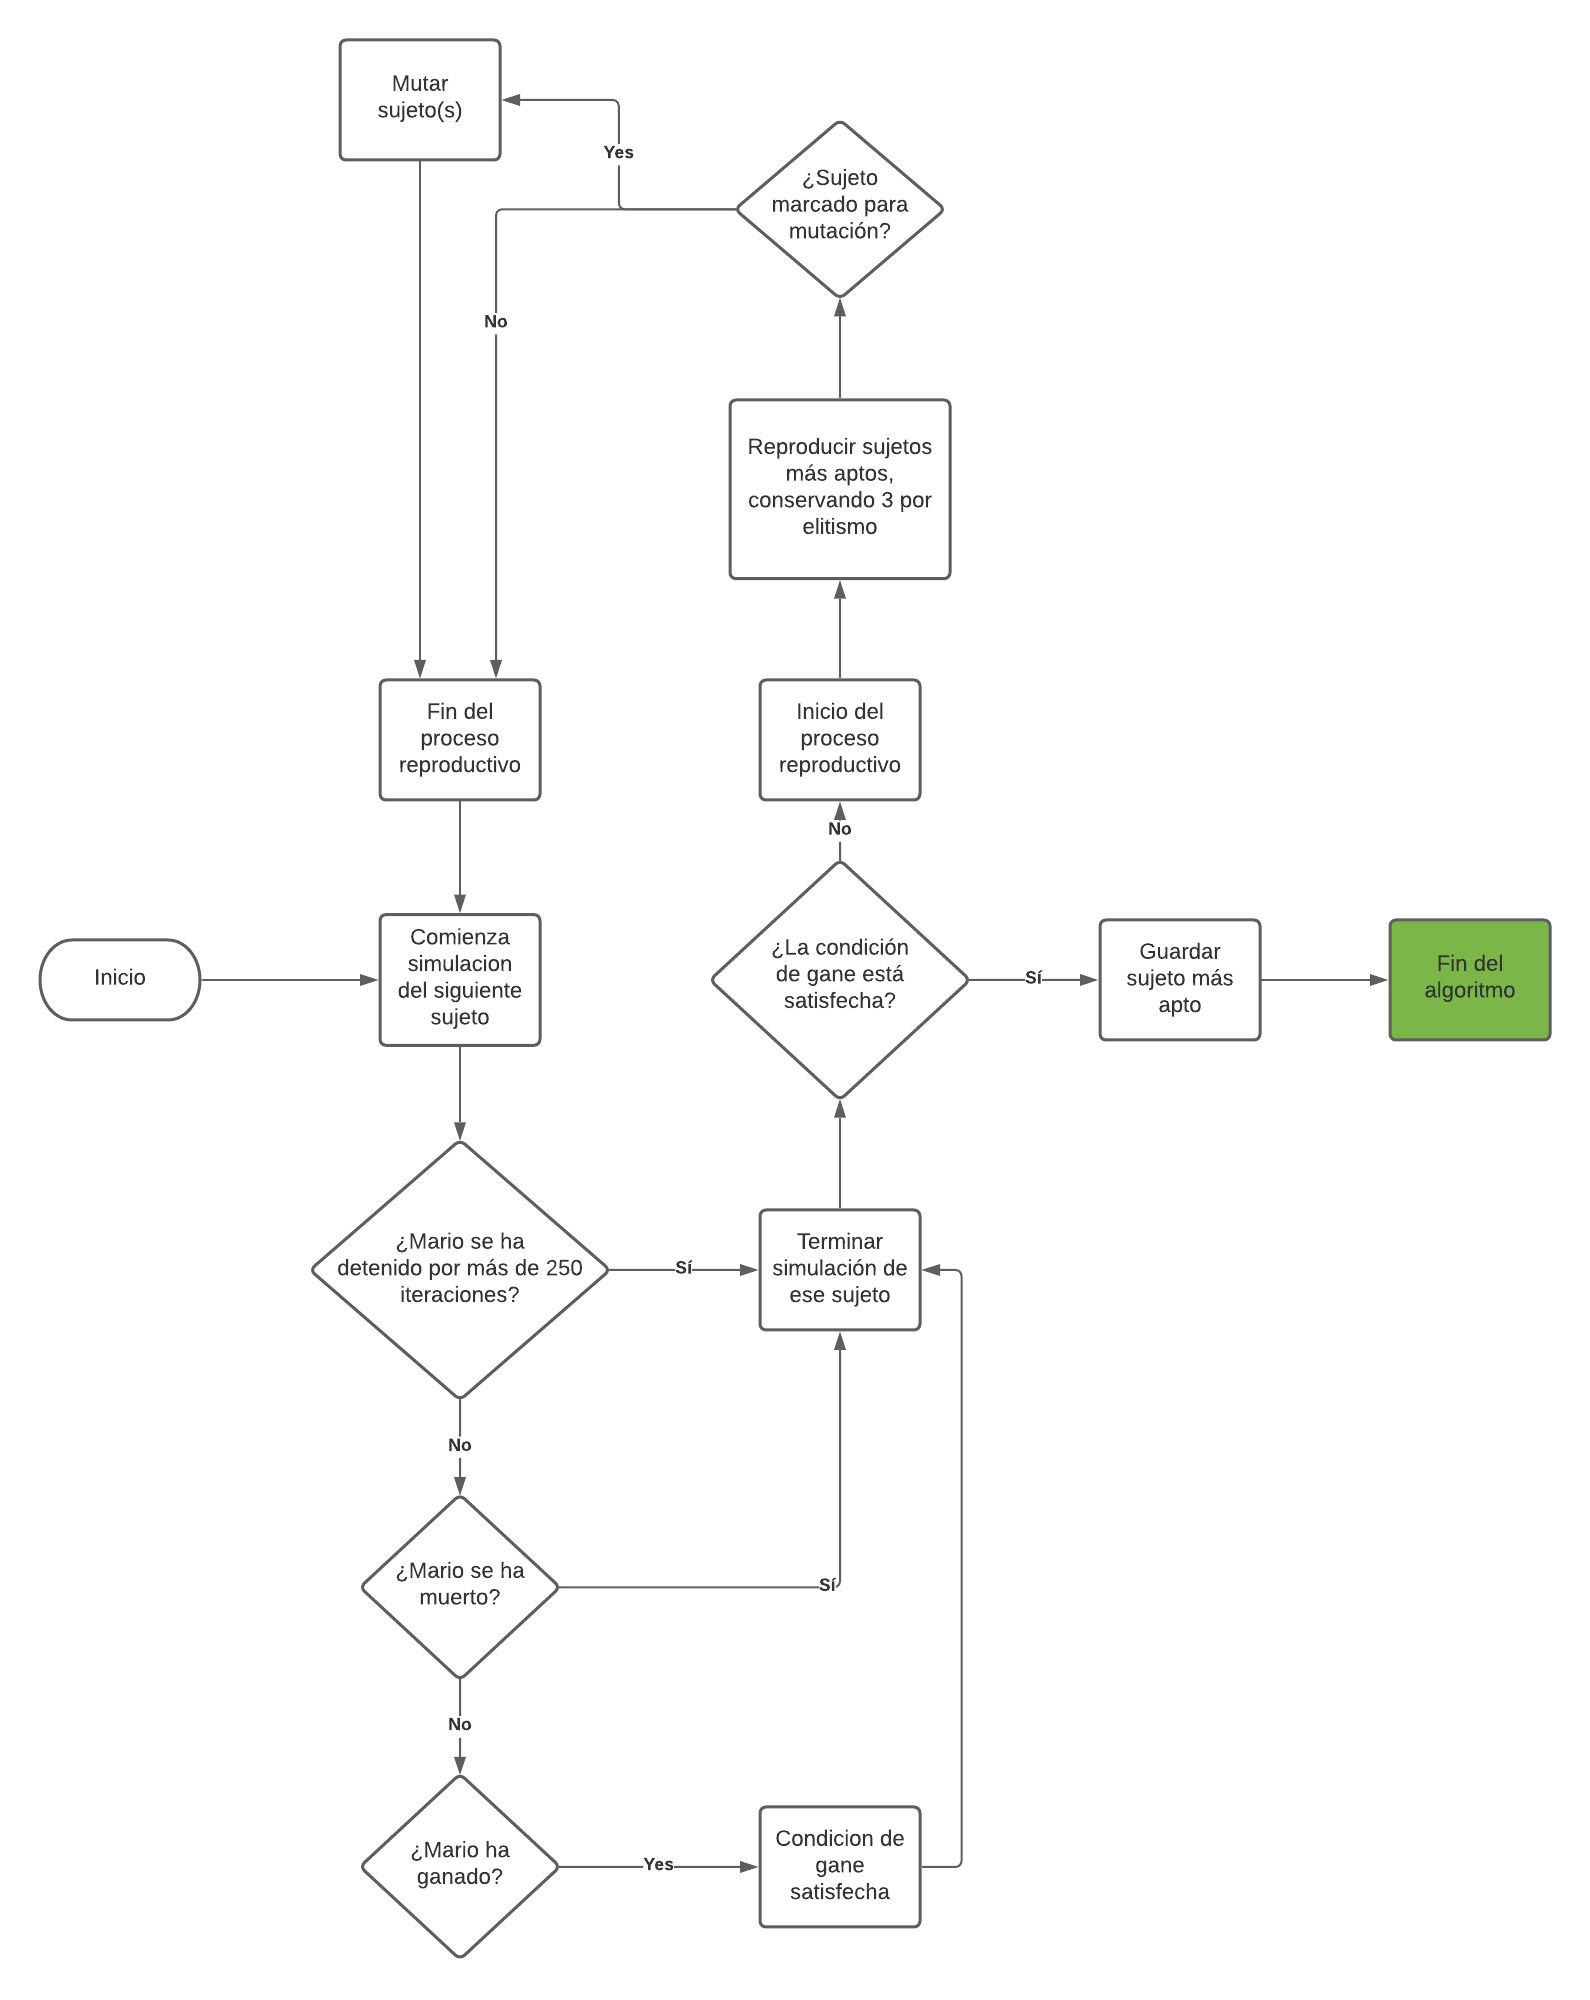
\includegraphics[scale=0.5]{neat/flujo.png}
\end{center}

\subsubsection{Estrategia de ramificación}
La estrategia de ramificación consiste en cruzar 147 individuos a partir de los padres más aptos (los que tienen el fitness más alto). El fitness se calcula a partir de qué tan lejos llega Mario en el nivel. También se aplica un elitismo de 3 individuos, para conservar sus genes en la siguiente generación. De esta forma se crea un árbol familiar progresivo que se va ramificando hacia la meta de fitness.

\subsubsection{Cruces genéticos realizados}
En este algoritmo se aplicó un single point crossover el cual utiliza un valor aleatorio de 50\% de probabilidad para definir cual mitad del gen se va a utilizar.
\begin{minted}[]{python}
def crossover(self, gene2):
    assert self.key == gene2.key

    new_gene = self.__class__(self.key)
    for a in self._gene_attributes:
        if random() > 0.5:
            setattr(new_gene, a.name, getattr(self, a.name))
        else:
            setattr(new_gene, a.name, getattr(gene2, a.name))

    return new_gene
\end{minted}
\textcite{neat-python}

\subsubsection{Tipo de mutación que se aplicó}
En este algoritmo se utiliza una mutación que obtiene el valor del cromosoma como dato de entrada. Luego, a partir de qué tan potente sea la mutación, según el archivo de configuración, se hace la mutación. La mutación consiste en conseguir el valor del cromosoma y sumarle un valor aleatorio entre cero y la potencia de mutación especificada. Una vez hecho esto, la función clamp de Pytorch se encarga de asegurarse que el tensor resultante esté en el rango de valores válidos.
\begin{minted}[]{python}
def mutate_value(self, value, config):
  mutate_rate = getattr(config, self.mutate_rate_name)
  # mutate_rate es especificado en el archivo de configuración
  # para este algoritmo tiene un valor de 5\%
  r = random()
  if r < mutate_rate:
      mutate_power = getattr(config, self.mutate_power_name)
      return self.clamp(value + gauss(0.0, mutate_power), config)

  replace_rate = getattr(config, self.replace_rate_name)

  if r < replace_rate + mutate_rate:
      return self.init_value(config)

  return value
\end{minted}
\textcite{neat-python}

\subsubsection{Función objetivo de la maximización de recursos}
Para maximizar los recursos computacionales, la pantalla del emulador se le baja la resolución, y se pasa a blanco y negro. Además se pasa a un arreglo unidimensional. Esto hace que la información por cada cuadro pueda ser interpretada de manera más fácil, por la red neuronal.
\begin{minted}[]{python}
def downscale_image(ob, size_x, size_y):
    ob = cv2.resize(ob, (size_x, size_y))
    ob = cv2.cvtColor(ob, cv2.COLOR_BGR2GRAY)
    ob = np.reshape(ob, (size_x, size_y))
    imgarray = np.ndarray.flatten(ob)
    return imgarray
\end{minted}

\subsubsection{Medición empírica}
\begin{center}
  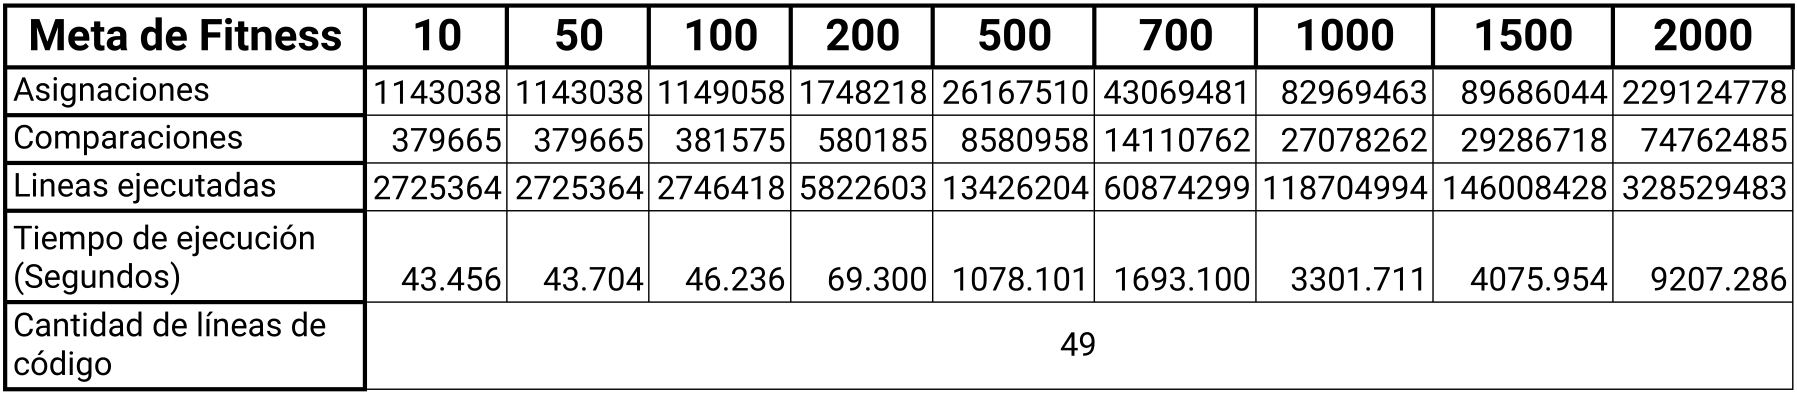
\includegraphics[scale=0.2]{neat/med-emp.png}
\end{center}

\subsubsection{Medición analítica}
\begin{minted}[]{python}
env = retro.make('SuperMarioBros-Nes', 'Level1-1') # 1

def downscale_image(ob, size_x, size_y):
    ob = cv2.resize(ob, (size_x, size_y)) # 1
    ob = cv2.cvtColor(ob, cv2.COLOR_BGR2GRAY) # 1
    ob = np.reshape(ob, (size_x, size_y)) # 1
    imgarray = np.ndarray.flatten(ob) # 1
    return imgarray # 1

def eval_genomes(genomes, config):
    for genome_id, genome in genomes: # 2n + 1
        ob = env.reset() # n+1

        size_x, size_y, img_color= env.observation_space.shape
        # n+1

        size_x = int(size_x/8) # n+1
        size_y = int(size_y/8) # n+1

        net = neat.nn.recurrent.RecurrentNetwork.create(genome, config)
        # n+1

        current_max_fitness = 0 # n
        fitness_current = 0 # n
        stag_counter = 0 # n

        xpos_lo = 0 # n
        xpos_hi = 0 # n

        done = False # n
        won = False # n

        while not done: # n^2+1
            imgarray = downscale_image(ob, size_x, size_y) #n^2

            nnOutput = net.activate(imgarray) #n^2

            ob, rew, done, info = env.step(nnOutput) #n^2

            xpos_lo = info['xscrollLo'] #n^2+1

            next_xpos_hi = info['xscrollHi'] #n^2+1

            if(next_xpos_hi > xpos_hi): #n^2
                xpos_hi = next_xpos_hi #n^2

            if xpos_hi >= 12 and not won: #2n^2
                fitness_current *= xpos_hi #n^2
                won = True #n^2
            else:
                fitness_current += rew #n^2

            if fitness_current > current_max_fitness: #n^2
                current_max_fitness = fitness_current #n^2
                stag_counter = 0 #n^2
            else:
                stag_counter += 1 #n^2

            if stag_counter > 250: #n^2
                done = True #n^2

            genome.fitness = fitness_current #n^2


\end{minted}

\textbf{Total(la suma de todos los pasos): \(18n^{2}+15n+15\)}


\textbf{Clasificación en notación O Grande: Cuadrática, \(O(n^{2})\)}

\subsubsection{Medición gráfica}
\begin{center}
  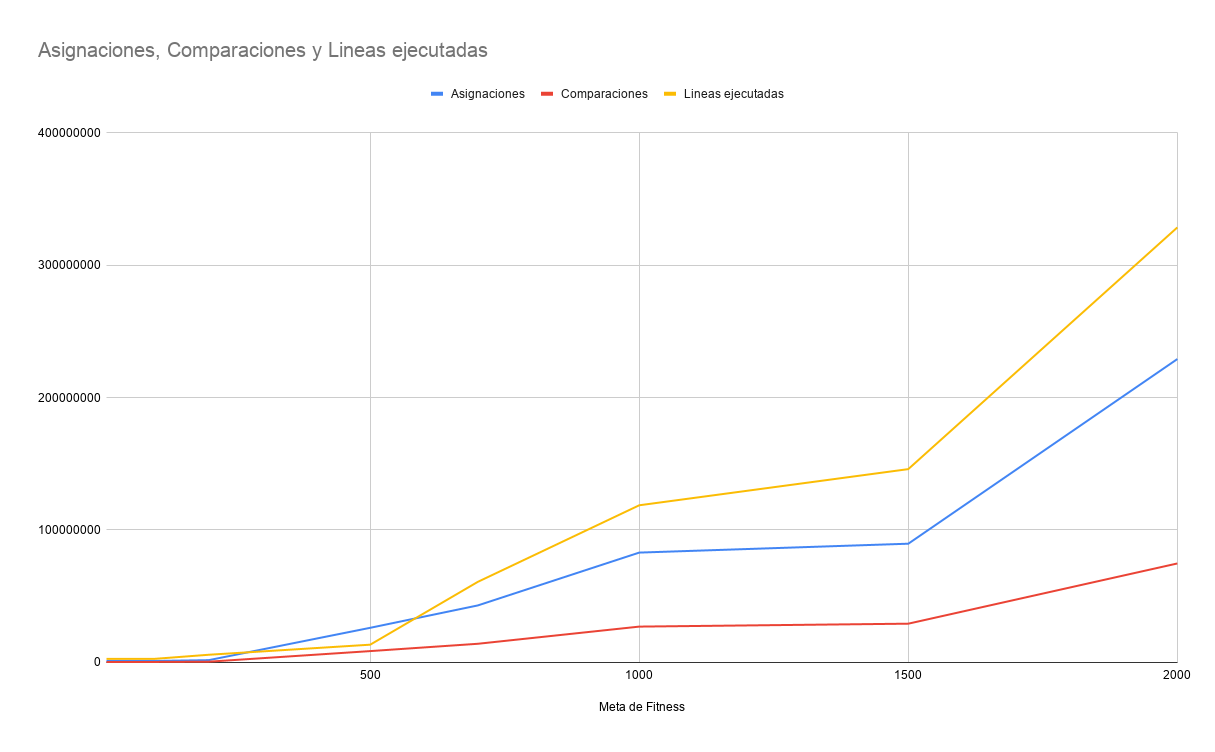
\includegraphics[scale=0.32]{neat/graf-acl.png}
  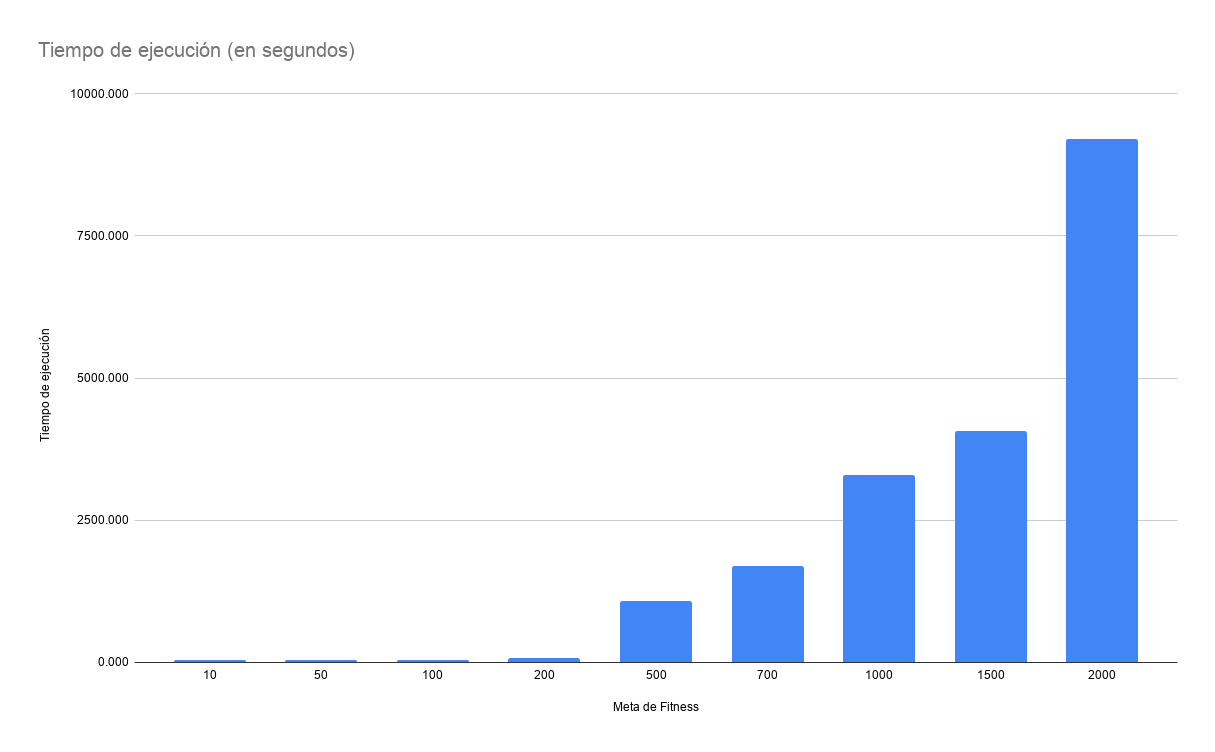
\includegraphics[scale=0.32]{neat/graf-time.png}
\end{center}

\subsubsection{Cálculo del factor de crecimiento}
\begin{center}
  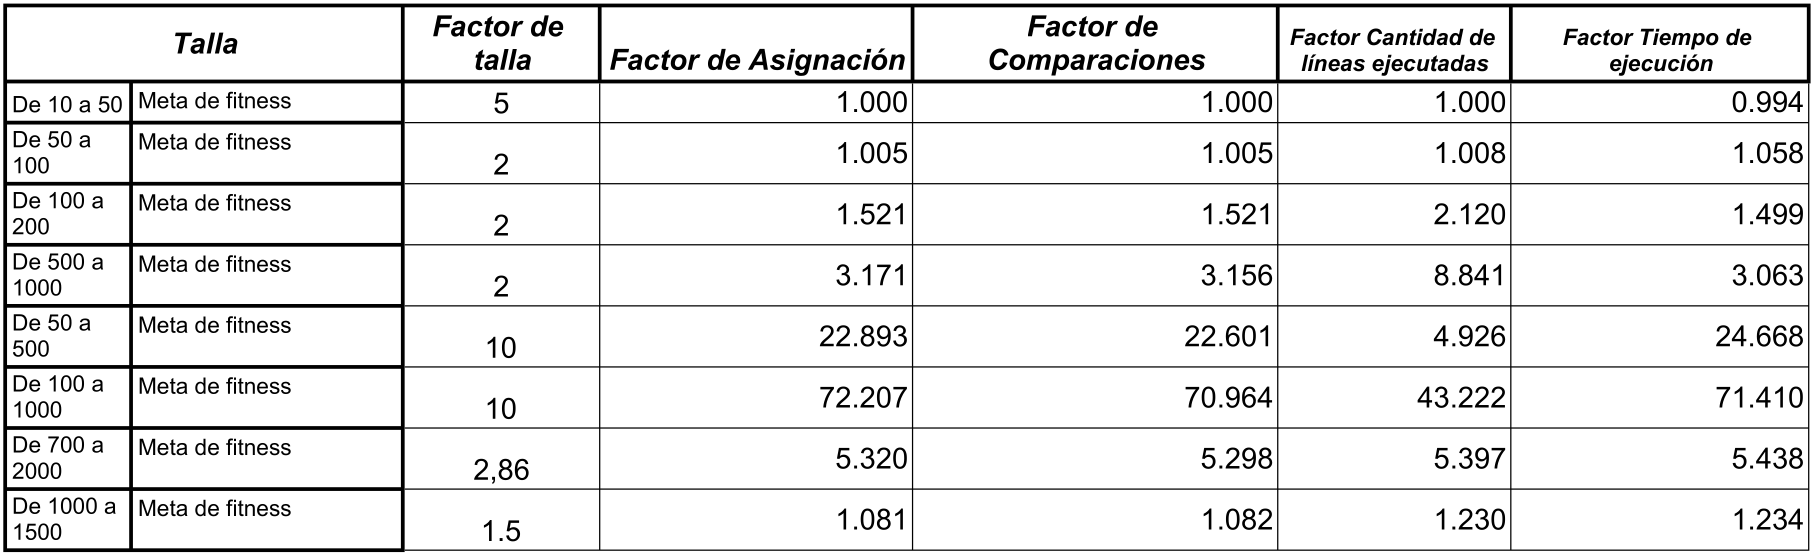
\includegraphics[scale=0.25]{neat/fac-crec.png}
\end{center}

Clasificación del comportamiento de las \textbf{asignaciones}: \(O(n^{2})\)

Clasificación del comportamiento de las \textbf{comparaciones}: \(O(n^{2})\)

%TODO
% \subsection{Clasificación según su entrada de los datos utilizando la notación O Grande, \(\Theta\) y \(\Omega\):}

% Nivel sin obstáculos: \(\Omega\)

% Nivel con cantidad moderada de obstáculos: \(\Theta\)

% Nivel con muchos obstáculos: O Grande
\newpage
\subsection{Algoritmo probabilístico}
\subsubsection{Requisitos para correr el algoritmo}
\begin{itemize}
  \item Python 3.8
  \item gym-retro
\end{itemize}

\subsubsection{Diagrama de flujo de estrategia}
\begin{center}
  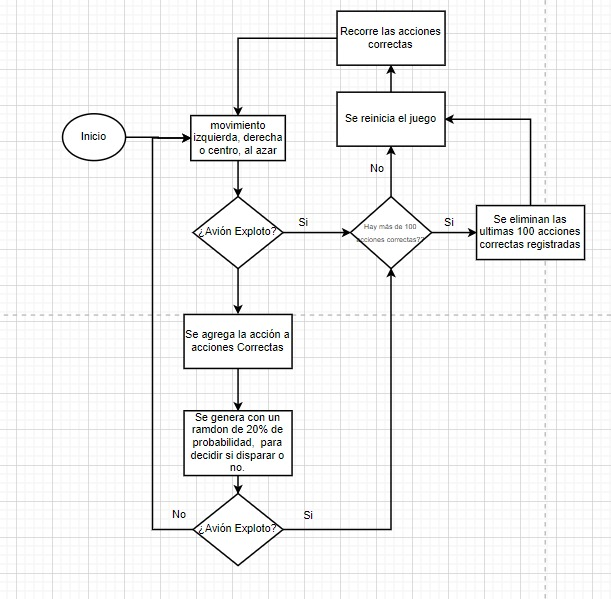
\includegraphics[scale=0.65]{prob/flujo.jpeg}
\end{center}

\subsubsection{Medición empírica}
\begin{center}
  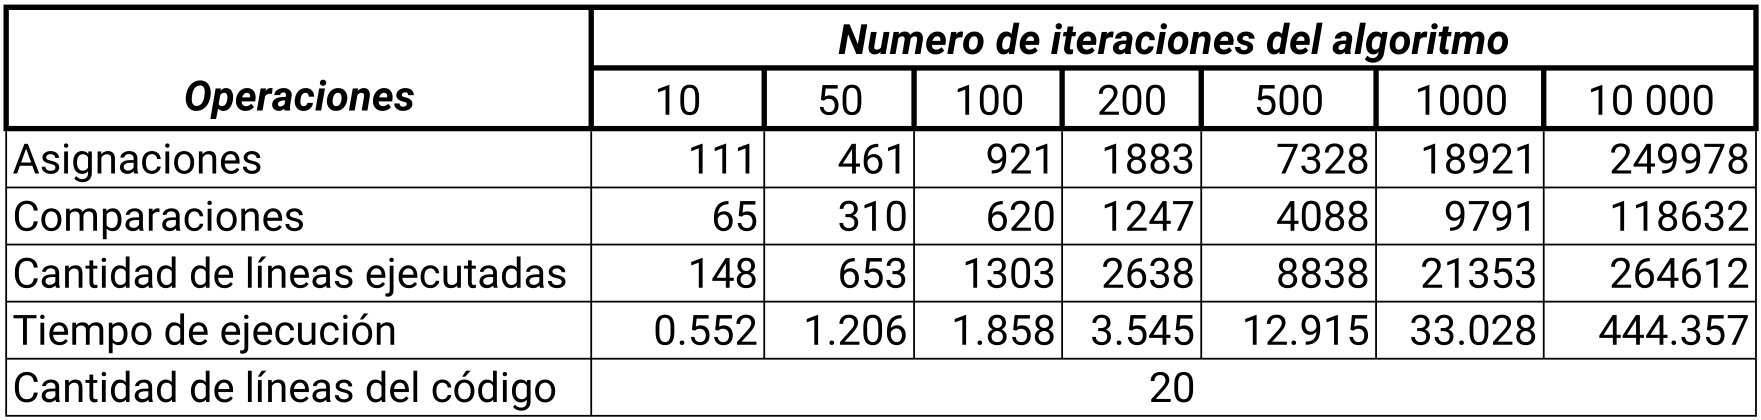
\includegraphics[scale=0.25]{prob/med-emp.png}
\end{center}

\subsubsection{Medición analítica}
\begin{minted}[]{python}
env = retro.make(game='Airstriker-Genesis', record=True) # 1
env.reset() # 1
done = False # 1
accionesCorrectas = [] # 1
iniciando = True # 1

while True: # n+1
    env.render() # n
    probabilidadDisparo = random() # n
    action = [0, 0, 0, 0, 0, 0, randint(0,1), randint(0,1), 0, 1, 0, 0] # n
    ob, rew, done, info = env.step(action) # n

    if iniciando and info['gameover'] ==9: # n
        iniciando = False # n
        for i in range(len(accionesCorrectas)): # n^2 + 2n
            env.render() # n^2
            ob, rew, done, info = env.step(accionesCorrectas[i]) # n^2
            if info['gameover'] ==2: # n^2
                break # n^2

    if info['gameover'] ==9: # n
        accionesCorrectas.append(action) # n
    if info['gameover'] ==2: # n
        iniciando = True # n
        obs = env.reset() # n
        if (len(accionesCorrectas)>100): # n
            for e in range(100): n^2+ 2n
                accionesCorrectas.pop(len(accionesCorrectas)-e-1) #n^2

    if probabilidadDisparo <= 0.20: #n
    action = [randint(0, 1), 0, 0, 0, 0, 0, randint(0, 1)
              , randint(0, 1), 0, 1, 0, 0] #n
        ob, rew, done, info = env.step(action) #n
        if info['gameover'] == 9: #n
            accionesCorrectas.append(action) #n

    if done: #n
        obs = env.reset() #n

env.close() #1
\end{minted}


\textbf{Total(la suma de todos los pasos): \(7n^{2}+24n+7\)}


\textbf{Clasificación en notación O Grande: Cuadrática, \(O(n^{2})\)}

\subsubsection{Medición gráfica}
\begin{center}
  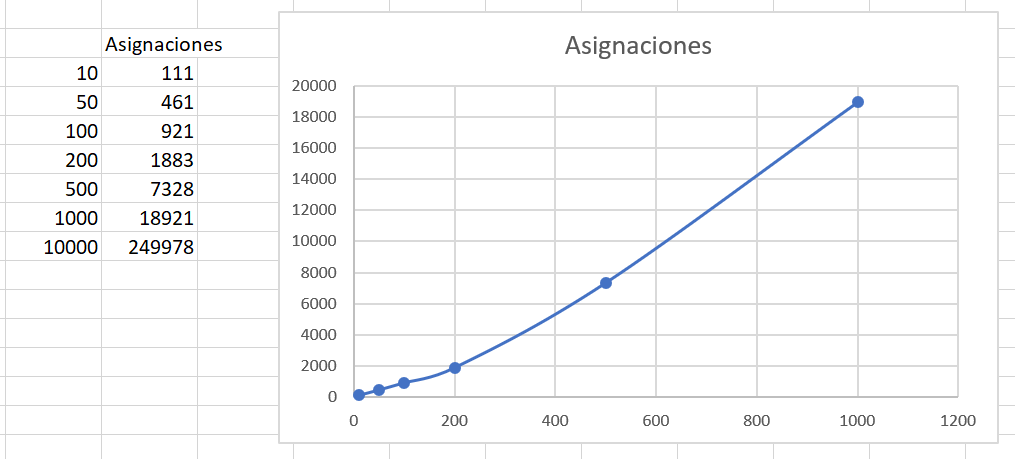
\includegraphics[scale=1.5]{prob/graf-asig.png}
\end{center}
\begin{center}
  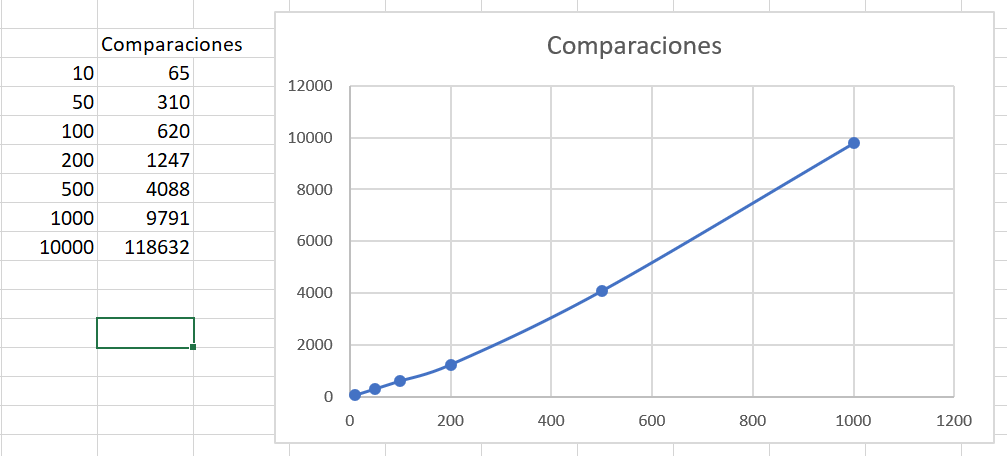
\includegraphics[scale=1.5]{prob/graf-comp.png}
\end{center}
\begin{center}
  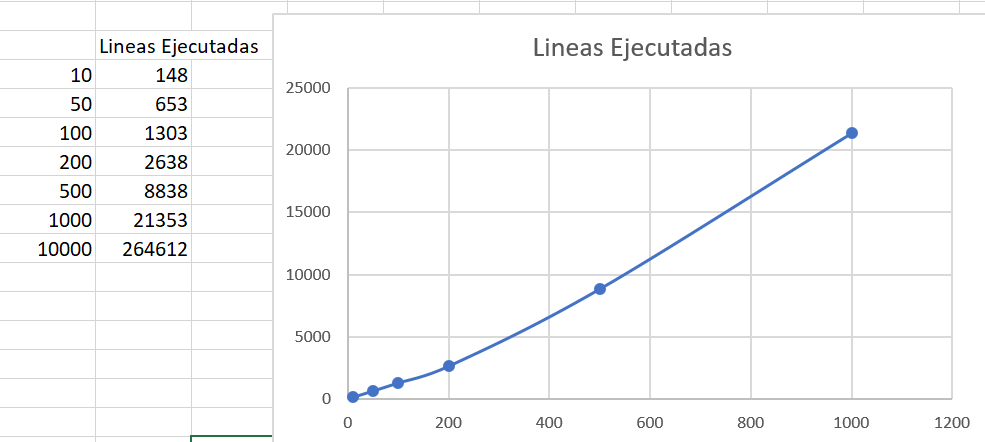
\includegraphics[scale=1.5]{prob/graf-lineas.png}
\end{center}

\subsubsection{Cálculo del factor de crecimiento}
\begin{center}
  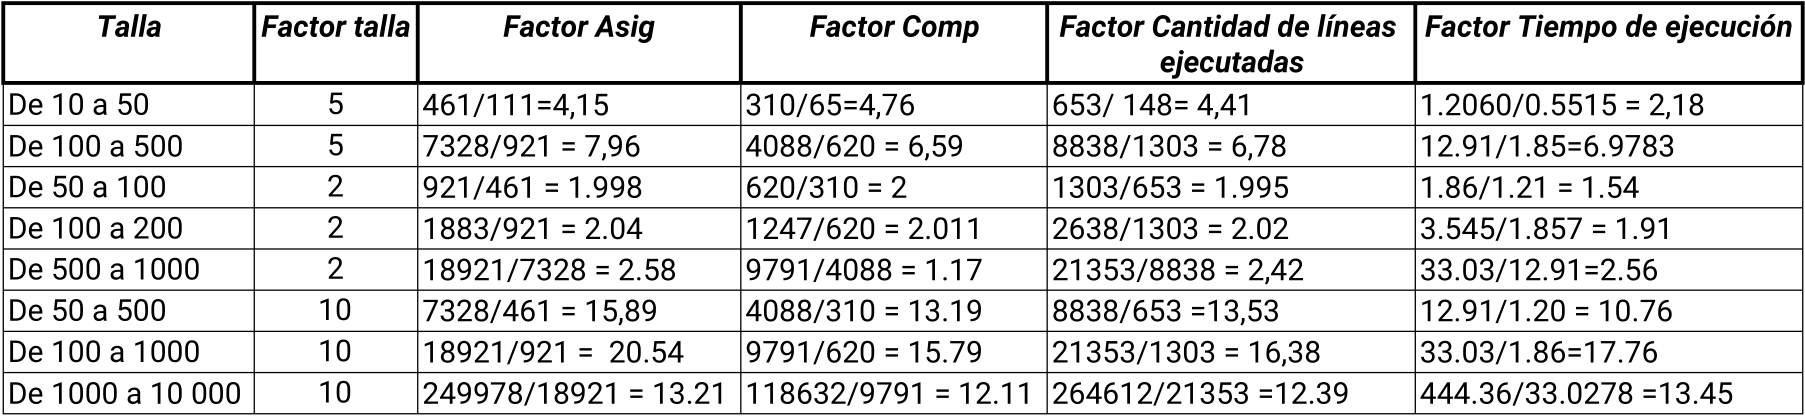
\includegraphics[scale=0.25]{prob/fac-crec.png}
\end{center}
\newpage
\section{Evaluación de resultados}
Una vez programados y analizados los algoritmos se ha llegado a la conclusión que ambos algoritmos tienen una complejidad en tiempo de tipo \textit{cuadrática}. Sin embargo, a la hora de medirlos, fue muy difícil hacer que el algoritmo logre ejecutarse de la peor manera. Es decir, si el comportamiento asintótico de ambos algoritmos está alrededor de \(O(n^{2})\), los algoritmos programados tuvieron un comportamiento por debajo de esta. La razón por la cual se dio este fenómeno es porque los algoritmos propuestos no se pueden medir de la misma forma en la que se miden los algoritmos de ordenamiento. Es decir, para medir estos algoritmos de la forma más eficiente posible es necesario utilizar otros métodos o herramientas.

Los resultados de las mediciones demuestran que para resolver los niveles de la forma más eficiente, el algoritmo NEAT es superior al algoritmo probabilístico. Esto es porque NEAT es un algoritmo más avanzado que puede generar soluciones más complejas que un algoritmo probabilístico. No obstante, NEAT requiere mucho tiempo de entrenamiento, por lo cual se argumenta que para niveles, o juegos más simples, el algoritmo probabilístico es superior a NEAT. Esto se debe a que por la naturaleza de los algoritmos probabilísticos, estos pueden dar una respuesta, más rápida, pero no necesariamente la más eficiente. Cabe resaltar que los algoritmos NEAT, por su complejidad, generan más overhead que los algoritmos probabilistas. Entonces, si no se dispone de hardware lo suficientemente potente para poder correr el algoritmo genético, este se podría volver intratable en tiempo. Este es otro ámbito en el que el algoritmo probabilístico es superior al genético.

\section{Conclusiones}
Después de pruebas extensas, para los objetivos propuestos al principio de esta investigación, se han obtenido resultados positivos. Dado que se lograron resolver los niveles propuestos, con los algoritmos propuestos.
Esto responde la pregunta del propósito principal de esta investigación: \textit{¿Es posible resolver niveles de videojuegos utilizando algoritmos probabilísticos y genéticos?} En este caso la respuesta es un \textbf{sí}. Para las preguntas específicas, en el caso de: ¿Qué tan demandantes son los algoritmos genéticos y probabilísticos en este caso de uso?, la respuesta es que como ambos algoritmos tienen una complejidad cuadrática, son moderadamente demandantes, pero aceptables. También quedó concluido que para juegos más complejos, los algoritmos genéticos dan mejores soluciones que los algoritmos probabilísticos. Sin embargo, el único objetivo que no se puede concluir del todo es si estos algoritmos son un reemplazo válido para los humanos. Por su complejidad y duración.
Sin embargo, la complejidad en tiempo de estos algoritmos hace que no sean más rápidos que los humanos resolviendo problemas simples. Sin embargo, para resolver problemas más amplios si se podría argumentar que los algoritmos probabilísticos y genéticos pueden ser más rápidos que los humanos.

\subsection{Recomendaciones, defectos y mejoras}
\subsubsection{Algoritmo genético}
Con respecto al algoritmo genético, solo hubo un defecto. La función de fitness propuesta no daba resultados consistentes. Por lo cual se tuvo que implementar una función de fitness que da resultados menos eficientes pero más consistentes. La función original le restaba el tiempo tomado al valor de fitness, para premiar más a los sujetos que duraran menos. Pero esto hacía que muchas veces los sujetos se quedaran estancados. La versión más simple de la función de fitness es solo premiar más entre más lejos llegue el sujeto en el eje \(x\).

Además, a continuación se proponen ciertas recomendaciones y mejoras:
\begin{itemize}
\item Hacer una nueva función de fitness que logre soluciones más eficientes. Esto se puede lograr utilizando valores exponenciales en vez de lineales en los valores de fitness, sin embargo, requiere más pruebas para comprobar que no se van a estancar la mayoría de los sujetos.
\item Probar con diferentes funciones de crossover para ver si se logran obtener resultados más eficientes y consistentes.
\item Probar con diferentes valores de configuración en la red neuronal.
\item Utilizar la librería de Tensor Flow, para hacer que el proceso de entrenamiento se más rápido utilizando un GPU.
\item Hacer pruebas con más niveles de Super Mario Bros. para lograr replicar el experimento con variables distintas.
\end{itemize}

\subsubsection{Algoritmo probabilístico}
Una vez concluido el proyecto, se considera interesante investigar sobre otros mecanismos relacionados con el machine learning y la AI, además se propone:
\begin{itemize}
\item Extender el estudio realizado en este proyecto acerca de los algoritmos probabilistas, para tratar de mejorar el rendimiento del algoritmo desarrollado en este trabajo o algoritmos similares.
\item Analizar con mayor detenimiento la forma de buscar soluciones aleatorias, para lograr abarcar más soluciones y lograr elegir entre la más adecuadas.
\item Entender las mediciones y estudios realizados a cada algoritmo para tener un panorama más claro de lo que se está realizando o de lo que se quiere realizar.
\item Tratar de dar la oportunidad de realizar la mayor cantidad de iteraciones o pruebas al algoritmo probabilístico, dado que los algoritmos probabilistas entre mas pruebas haga, mayor será su posibilidad de ganar.
\end{itemize}

\printbibliography{}

\end{document}
